\section{Introdução}

\begin{figure}
    \centering 
    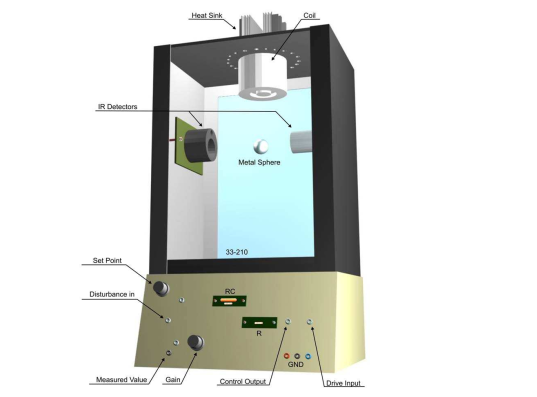
\includegraphics[width=\linewidth]{Unidade_MagLev.png}
    \caption{Unidade de Levitação Magnética [1]}
    \label{fig:1}
\end{figure}

A levitação magnética é um fenômeno físico no qual um objeto é sustentado no espaço sem contato físico com uma superfície, utilizando apenas forças magnéticas. Essa técnica se baseia no princípio de que polos magnéticos opostos se atraem, enquanto polos iguais se repelem, permitindo que campos magnéticos sejam empregados para suspender objetos contra a força da gravidade. Sistemas de levitação magnética apresentam diversas aplicações, como trens Maglev de alta velocidade, rolamentos magnéticos, que se beneficiam da ausência de contato físico, resultando em baixo atrito no rolamento. A unidade de levitação magnética possui em sua base a interface de conexão, sobre a qual está montada a unidade mecânica em que a bobina produzirá os efeitos magnéticos. Ela apresenta um sensor infra-vermelho em ambas as laterais da unidade, além da esfera magnética, vide Figura 1.Nesse contexto, o estudo e desenvolvimento de controle para esses sistemas mostram-se fundamentais para possibilitar aplicações práticas. Assim, este trabalho propões a análise e controle de um sistema de levitação magnética utilizando métodos clássicos de controle, com o objetivo de regulação em ponto de operação da esfera pela unidade de levitação magnética.

